\documentclass[dvipdfmx]{jsarticle}
\usepackage{url}
\usepackage{listings}
\usepackage[dvipdfmx]{graphicx}
\usepackage{here}
\usepackage{ascmac}\usepackage{listings, jlisting, color}
\definecolor{OliveGreen}{rgb}{0.0,0.6,0.0}
\definecolor{Orenge}{rgb}{0.89,0.55,0}
\definecolor{SkyBlue}{rgb}{0.28, 0.28, 0.95}
\lstset{
  language={C++}, % 言語の指定
  basicstyle={\ttfamily},
  identifierstyle={\small},
  commentstyle={\smallitshape},
  keywordstyle={\small\bfseries},
  ndkeywordstyle={\small},
  stringstyle={\small\ttfamily},
  frame={tb},
  breaklines=true,
  columns=[l]{fullflexible},
  numbers=left,
  xrightmargin=0zw,
  xleftmargin=3zw,
  numberstyle={\scriptsize},
  stepnumber=1,
  numbersep=1zw,
  lineskip=-0.5ex,
  keywordstyle={\color{SkyBlue}},     %キーワード(int, ifなど)の書体指定
  commentstyle={\color{OliveGreen}},  %注釈の書体
  stringstyle=\color{Orenge}          %文字列
}

\begin{document}
\title{ロボ部(仮)資料案}
\author{かちがわの杜 舟橋}
\maketitle

\section{はじめに}
高校数学アルゴリズムをプログラミングを使って解くコンセプトなロボ部の資料案.\\
アルゴリズムを学習することで高校数学の習熟を手助けすることはもちろん,様々な問題の答えに効率的にたどり着くことができると考える.
\section{数学I+A,II+B単元一覧\cite{tangen}}
数学I+A,II+B単元一覧です.\\
数学Iでプログラミングを使って解くことのできそうな単元
\begin{figure}[H]
  \centering
  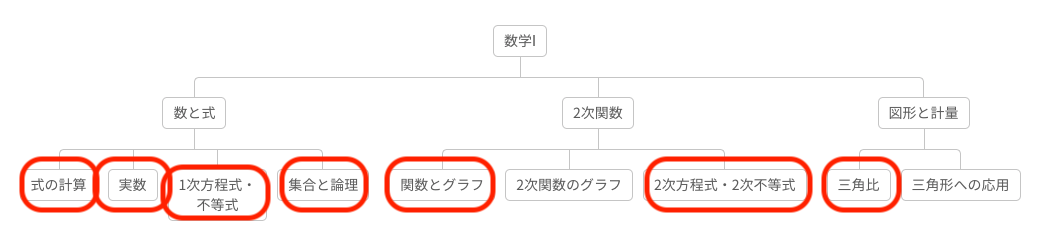
\includegraphics[width=15cm]{1.png}
  \caption{数学I}
\end{figure}
数学Aでプログラミングを使って解くことのできそうな単元
\begin{figure}[H]
  \centering
  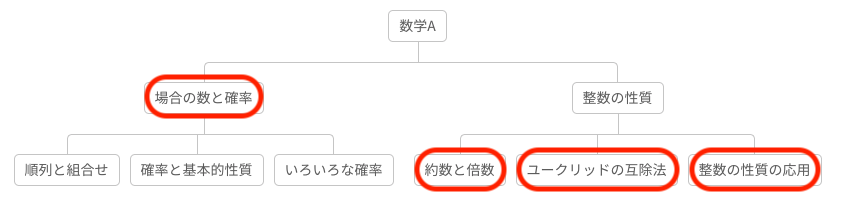
\includegraphics[width=15cm]{A.png}
  \caption{数学A}
\end{figure}
数学IIでプログラミングを使って解くことのできそうな単元
\begin{figure}[H]
  \centering
  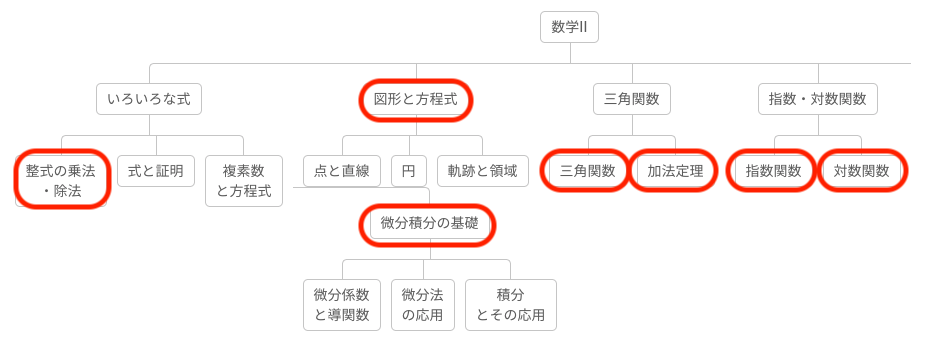
\includegraphics[width=15cm]{2.png}
  \caption{数学II}
\end{figure}
数学Bでプログラミングを使って解くことのできそうな単元
\begin{figure}[H]
  \centering
  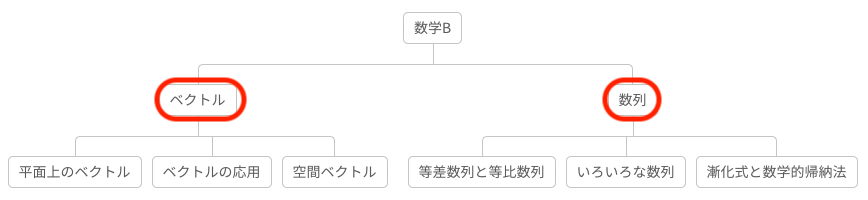
\includegraphics[width=15cm]{B.png}
  \caption{数学B}
\end{figure}
\section{問題例}
\subsection{数学A 約数と倍数,数学B 数列}
すぬけ君は,黒板に書かれている整数がすべて偶数であるとき,書かれている整数すべてを2で割ったものに置き換える事ができます.
任意の数字を入力して,すぬけ君は最大で何回操作を行うことができるかを求めよう!\cite{atcoder}
\subsection{数学A 場合の数}
もつお君は,500円玉をA枚,100円玉をB枚,50円玉をC枚持っています.これらの硬貨の中から何枚かを選び,合計金額をちょうどX円にする方法は何通りあるか調べよう!同じ種類の硬貨どうしは区別できません.2 通りの硬貨の選び方は,ある種類の硬貨についてその硬貨を選ぶ枚数が異なるとき区別されます.\cite{atcoder}
\begin{thebibliography}{99}
\bibitem{tangen} suugaku.jp 高校数学単元表 :(\url{https://suugaku.jp/range.php})
\bibitem{atcoder} AtCoder:(\url{https://atcoder.jp/})
\bibitem{monkasyo} 文部科学省(2017)小学校段階におけるプログラミング教育の在り方について(議論の取りまとめ),文部科学省:(\url{http://www.mext.go.jp/b_menu/shingi/chousa/shotou/122/attach/1372525.htm})
Access
\end{thebibliography}

\end{document}